% ecoLocator architecture figure (polygenic-score network).
% Compile: pdflatex EcolocatorARC_pgs.tex
\RequirePackage{fix-cm}
\documentclass[tikz,border=2pt]{standalone}
\usepackage[T1]{fontenc}
\usepackage{lmodern}
\usepackage{helvet}
\renewcommand{\familydefault}{\sfdefault}
\usepackage{sansmath}
\sansmath
\usetikzlibrary{arrows.meta}

\definecolor{train}{HTML}{6E83CA}
\definecolor{pred}{HTML}{F9A80E}
\definecolor{rain}{HTML}{2E3192}
\definecolor{mesh}{gray}{0.62}
\definecolor{note}{gray}{0.35}

\newcommand{\fs}[1]{\fontsize{#1}{#1pt}\selectfont}

\tikzset{
  unit/.style={draw=black!70, line width=0.4pt, fill=white},
  keyunit/.style={draw=black, line width=0.6pt, fill=white},
  drop/.style={draw=black!45, line width=0.4pt, dashed, fill=white},
  meshline/.style={draw=mesh, line width=0.2pt},
  flow/.style={draw=black, line width=0.6pt, -{Stealth[length=4pt,width=3.5pt]}},
  plain/.style={draw=black, line width=0.6pt},
  gate/.style={draw=black, line width=0.9pt},
  card/.style={draw=black!55, line width=0.5pt, fill=white, rounded corners=2pt},
  cardback/.style={draw=black!35, line width=0.4pt, fill=white, rounded corners=2pt},
  group/.style={draw=black!55, line width=0.4pt, fill=white, rounded corners=2pt},
  lbl/.style={font=\fs{6.5}, text=note, inner sep=0pt},
  utxt/.style={font=\fs{6.5}, inner sep=0pt},
  bigarrow/.style={line width=1.2pt, -{Stealth[length=5pt,width=4.5pt]}},
}

% \ubox{x}{y}{width}{height}{style}{text}: a unit drawn as a rectangle from
% coordinates (not as a node), so that it shrinks with a scaled scope.
\newcommand{\ubox}[6]{%
  \draw[#5] ({#1-#3/2},{#2-#4/2}) rectangle ({#1+#3/2},{#2+#4/2});
  \node[utxt] at ({#1},{#2}) {#6};}

% Layer geometry. Each layer has five slots; slot 3 holds an ellipsis that
% stands for the units that are not drawn.
\newcommand{\slotx}[1]{(4.3+0.65*(#1-1))}
\def\yin{7.55}
\def\yA{6.75}
\def\yB{6.05}
\def\yC{5.35}
\def\yD{4.65}
\def\yloc{3.95}
\def\uw{0.42}
\def\uh{0.30}

% \mesh{y of upper layer}{y of lower layer}{dropped slot of upper layer}
% A dropped unit sends nothing to the next layer.
\newcommand{\mesh}[3]{%
  \foreach \i in {1,2,4,5} {
    \ifnum\i=#3\else
      \foreach \j in {1,2,4,5} {
        \draw[meshline] ({\slotx{\i}},{#1-\uh/2}) -- ({\slotx{\j}},{#2+\uh/2});
      }
    \fi
  }}

% \layer{y}{dropped slot}
\newcommand{\layer}[2]{%
  \foreach \i in {1,2,4,5} {
    \ifnum\i=#2
      \ubox{\slotx{\i}}{#1}{\uw}{\uh}{drop}{}
    \else
      \ubox{\slotx{\i}}{#1}{\uw}{\uh}{unit}{}
    \fi
  }
  \node[utxt] at ({\slotx{3}},#1) {$\cdots$};}

% \net{1}: the network with labels; \net{0}: the same drawing without text.
\newcommand{\net}[1]{%
  \def\lt##1{\ifnum#1=1 ##1\fi}%
  % trunk meshes, behind the units
  \mesh{\yin}{\yA}{2}
  \mesh{\yA}{\yB}{4}
  \mesh{\yB}{\yC}{1}
  \mesh{\yC}{\yD}{5}
  \foreach \i in {1,4,5} {
    \foreach \j in {5.275,5.925} {
      \draw[meshline] ({\slotx{\i}},{\yD-\uh/2}) -- (\j,{\yloc+0.16});
    }
  }
  % input: standardized genotypes; the dashed unit is dropped
  \ubox{\slotx{1}}{\yin}{0.58}{\uh}{unit}{\lt{$-1.2$}}
  \ubox{\slotx{2}}{\yin}{0.58}{\uh}{drop}{\lt{\textcolor{black!45}{$0.4$}}}
  \ubox{\slotx{4}}{\yin}{0.58}{\uh}{unit}{\lt{$1.1$}}
  \ubox{\slotx{5}}{\yin}{0.58}{\uh}{unit}{\lt{$-0.3$}}
  \node[utxt] at ({\slotx{3}},\yin) {$\cdots$};
  % four dense layers, dropout after each
  \layer{\yA}{4}
  \layer{\yB}{1}
  \layer{\yC}{5}
  \layer{\yD}{2}
  % location head
  \ubox{5.275}{\yloc}{\uw}{0.32}{keyunit}{\lt{\fs{7}$x$}}
  \ubox{5.925}{\yloc}{\uw}{0.32}{keyunit}{\lt{\fs{7}$y$}}
  % environment route: one card per covariate
  \foreach \o in {0.24,0.12} {
    \draw[cardback] (8.95+\o,1.05+\o) rectangle (11.85+\o,6.3+\o);
  }
  \draw[card] (8.95,1.05) rectangle (11.85,6.3);
  % bypass: every input unit feeds the score unit directly
  \foreach \i in {1,2,4,5} {
    \draw[plain] ({\slotx{\i}},{\yin+\uh/2}) -- ({\slotx{\i}},7.9);
  }
  \draw[plain] ({\slotx{1}},7.9) -- (9.4,7.9);
  \draw[flow] (9.4,7.9) -- (9.4,5.6);
  % score unit
  \ubox{9.4}{5.42}{0.62}{0.34}{keyunit}{\lt{\fs{7}$s_j$}}
  % correction head: a small dense layer, then one linear unit
  \draw[group] (8.98,3.72) rectangle (10.12,4.22);
  \foreach \cx in {9.15,9.42,9.95} {
    \draw[meshline] (\cx,3.86) -- (9.65,3.12);
  }
  \ubox{9.15}{3.97}{0.2}{0.2}{unit}{}
  \ubox{9.42}{3.97}{0.2}{0.2}{unit}{}
  \node[utxt] at (9.685,3.97) {\lt{\fs{4.5}$\cdots$}};
  \ubox{9.95}{3.97}{0.2}{0.2}{unit}{}
  \ubox{9.65}{2.95}{0.62}{0.34}{keyunit}{\lt{\fs{7}$h_j$}}
  % score into the correction head and, with coefficient 1, into the sum
  \draw[flow] (9.4,5.25) -- (9.4,4.24);
  \draw[plain] (9.4,4.85) -- (11.3,4.85);
  \draw[flow] (11.3,4.85) -- (11.3,3.14);
  % predicted location into the correction head, through a gradient stop
  \draw[flow] (6.14,\yloc) -- (8.96,\yloc);
  \fill[white] (7.63,3.8) rectangle (7.77,4.1);
  \draw[gate] (7.62,3.8) -- (7.62,4.1);
  \draw[gate] (7.78,3.8) -- (7.78,4.1);
  % correction into the sum; sum to the output
  \draw[flow] (9.96,2.95) -- (11.13,2.95);
  \draw[plain, fill=white] (11.3,2.95) circle (0.17);
  \draw[plain] (11.2,2.95) -- (11.4,2.95) (11.3,2.85) -- (11.3,3.05);
  \draw[flow] (11.3,2.78) -- (11.3,2.12);
  \ubox{11.3}{1.92}{0.72}{0.34}{keyunit}{\lt{env $j$}}
  % labels
  \ifnum#1=1
    \node[font=\fs{7.5}, anchor=south, inner sep=0pt] at (5.6,8.08) {Standardized genotypes};
    \node[lbl, anchor=west] at (7.35,\yin) {input dropout 0.1};
    \node[lbl, anchor=west] at (9.5,7.05) {all SNPs};
    \node[lbl, anchor=west, align=left] at (7.2,5.7)
      {4 dense layers\\[1pt]128 units, ELU\\[1pt]dropout 0.25};
    \node[lbl, anchor=east, align=right] at (5.0,\yloc) {Location\\[1pt]head};
    \node[lbl, anchor=north] at (7.7,3.72) {no gradient};
    \node[font=\fs{7}, anchor=west, inner sep=0pt] at (9.82,5.53) {Polygenic score};
    \node[lbl, anchor=west] at (9.82,5.24) {linear, no bias, L2};
    \node[lbl, anchor=west, align=left] at (10.2,3.97) {16 units\\[1pt]ELU};
    \node[font=\fs{7}, anchor=north, inner sep=0pt] at (9.65,2.66) {Correction head};
    \node[lbl, anchor=west] at (11.38,3.4) {1};
    \node[lbl, anchor=south west, align=left] at (9.0,1.2)
      {one route per\\[1pt]covariate (env 1--3)};
  \fi
}

% \genomat{x0}{y top}{rows}: three individuals by five SNPs; each individual
% shows its two haplotypes, one above the other.
\newcommand{\genomat}[3]{%
  \begin{scope}[shift={(#1,#2)}]
    \foreach \r/\row in {#3} {
      \foreach \c/\a/\b in \row {
        \node[font=\fs{7.5}, inner sep=0pt] at ({0.25+0.5*(\c-1)},{-0.6*(\r-1)-0.16}) {\a};
        \node[font=\fs{7.5}, inner sep=0pt] at ({0.25+0.5*(\c-1)},{-0.6*(\r-1)-0.44}) {\b};
      }
      \draw[black!50, line width=0.4pt, densely dotted] (0,{-0.6*(\r-1)-0.3}) -- (2.5,{-0.6*(\r-1)-0.3});
    }
    \foreach \c in {1,2,3,4} { \draw[black!60, line width=0.4pt] ({0.5*\c},0) -- ({0.5*\c},-1.8); }
    \foreach \r in {1,2} { \draw[black, line width=1pt] (0,{-0.6*\r}) -- (2.5,{-0.6*\r}); }
    \draw[black, line width=1.2pt] (0,0) rectangle (2.5,-1.8);
  \end{scope}}

% Sun and rain symbols for the environment.
\newcommand{\sunicon}[3]{% x, y, radius
  \begin{scope}[shift={(#1,#2)}]
    \draw[pred, line width=0.6pt, fill=white] (0,0) circle (#3);
    \foreach \t in {0,45,...,315} {
      \draw[pred, line width=0.6pt] (\t:{#3*1.35}) -- (\t:{#3*1.85});
    }
  \end{scope}}
\newcommand{\raindrop}[2]{% x, y of the tip
  \fill[rain] (#1,#2) .. controls ({#1-0.02},{#2-0.05}) and ({#1-0.055},{#2-0.09}) ..
    ({#1-0.055},{#2-0.125}) arc[start angle=180, end angle=360, radius=0.055]
    .. controls ({#1+0.055},{#2-0.09}) and ({#1+0.02},{#2-0.05}) .. (#1,#2);}
\newcommand{\rainicon}[2]{\raindrop{#1}{#2}\raindrop{#1+0.14}{#2+0.07}}

\begin{document}
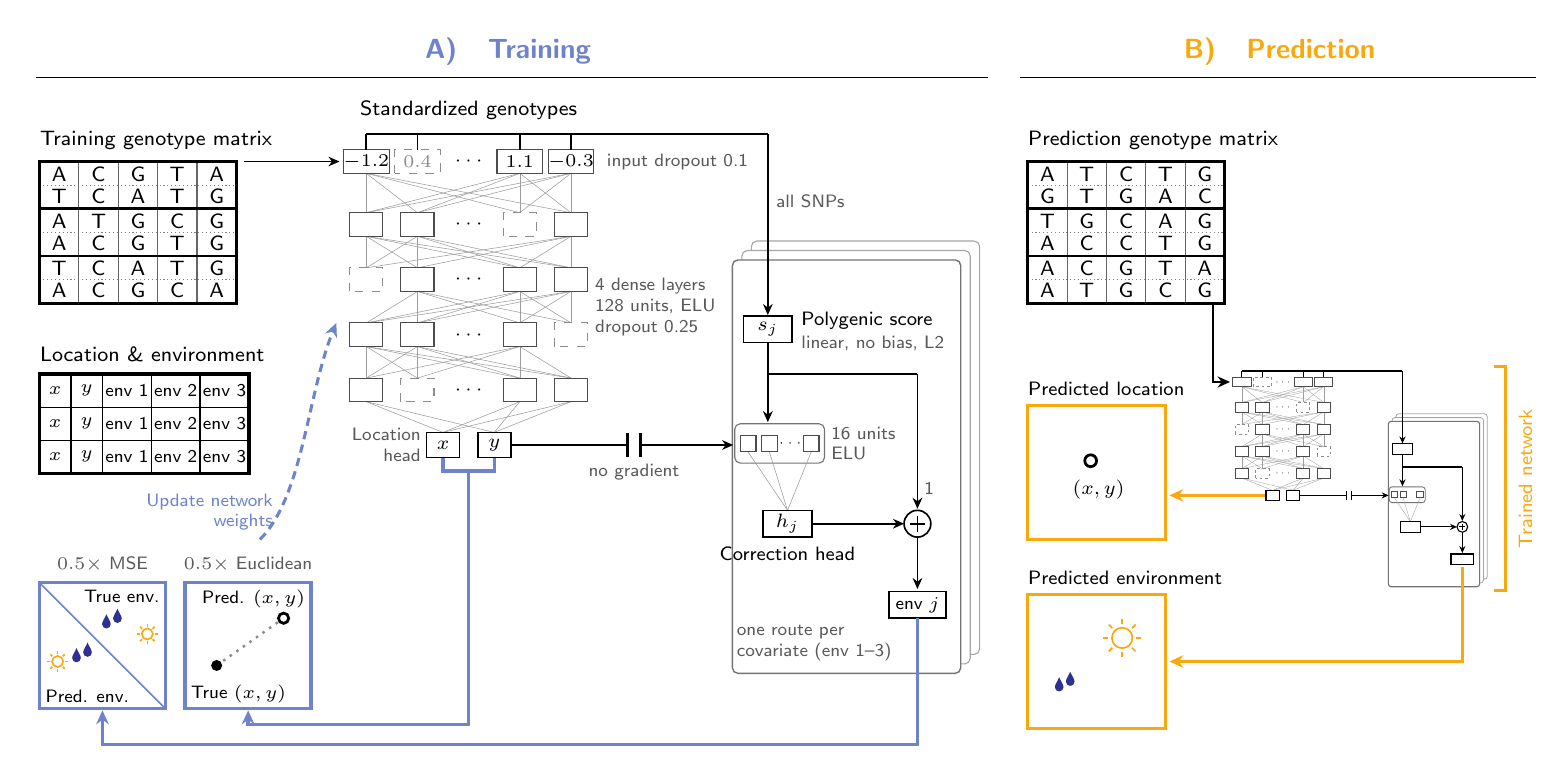
\begin{tikzpicture}[x=1cm,y=1cm]
  \useasboundingbox (0,0) rectangle (19.2,9.25);

  % ---------------- panel titles ----------------
  \node[font=\fs{10}\bfseries, text=train] at (6.1,8.95) {A)\quad Training};
  \draw[black, line width=0.4pt] (0.1,8.62) -- (12.2,8.62);
  \node[font=\fs{10}\bfseries, text=pred] at (15.9,8.95) {B)\quad Prediction};
  \draw[black, line width=0.4pt] (12.6,8.62) -- (19.15,8.62);

  % ---------------- A) training ----------------
  \node[font=\fs{7.5}, anchor=south west, inner sep=0pt] at (0.15,7.7) {Training genotype matrix};
  \genomat{0.15}{7.55}{1/{1/A/T,2/C/C,3/G/A,4/T/T,5/A/G},
                       2/{1/A/A,2/T/C,3/G/G,4/C/T,5/G/G},
                       3/{1/T/A,2/C/C,3/A/G,4/T/C,5/G/A}}

  % location and environment of the training samples
  \node[font=\fs{7.5}, anchor=south west, inner sep=0pt] at (0.15,5.0) {Location \& environment};
  \begin{scope}[shift={(0.15,4.85)}]
    \foreach \r in {0,1,2} {
      \foreach \x/\w/\t in {0/0.4/$x$,0.4/0.4/$y$,0.8/0.62/env 1,1.42/0.62/env 2,2.04/0.62/env 3} {
        \draw[black, line width=0.5pt] (\x,{-0.42*\r}) rectangle ({\x+\w},{-0.42*(\r+1)});
        \node[font=\fs{6.5}, inner sep=0pt] at ({\x+\w/2},{-0.42*\r-0.21}) {\t};
      }
    }
    \draw[black, line width=1.2pt] (0,0) rectangle (2.66,-1.26);
  \end{scope}

  \draw[flow] (2.75,\yin) -- (3.96,\yin);
  \net{1}

  % losses
  \node[lbl, anchor=south] at (0.95,2.33) {$0.5\times$ MSE};
  \node[lbl, anchor=south] at (2.8,2.33) {$0.5\times$ Euclidean};
  % environment loss
  \draw[train, line width=1.2pt] (0.15,0.6) rectangle (1.75,2.2);
  \draw[train, line width=0.6pt] (0.15,2.2) -- (1.75,0.6);
  \node[font=\fs{6.5}, anchor=north east, inner sep=0pt] at (1.68,2.12) {True env.};
  \rainicon{1.0}{1.8}
  \sunicon{1.52}{1.55}{0.07}
  \node[font=\fs{6.5}, anchor=south west, inner sep=0pt] at (0.22,0.67) {Pred. env.};
  \sunicon{0.38}{1.2}{0.07}
  \rainicon{0.62}{1.37}
  % location loss
  \draw[train, line width=1.2pt] (2.0,0.6) rectangle (3.6,2.2);
  \draw[black!45, line width=0.9pt, dotted] (2.4,1.15) -- (3.25,1.75);
  \fill[black] (2.4,1.15) circle (0.07);
  \draw[black, line width=1pt, fill=white] (3.25,1.75) circle (0.065);
  \node[font=\fs{6.5}, anchor=north east, inner sep=0pt] at (3.53,2.12) {Pred. $(x,y)$};
  \node[font=\fs{6.5}, anchor=south west, inner sep=0pt] at (2.07,0.67) {True $(x,y)$};

  % outputs to the losses; the two routes are nested and do not cross
  \draw[train, line width=1.2pt] (5.275,3.79) -- (5.275,3.62) -- (5.925,3.62) -- (5.925,3.79);
  \draw[train, bigarrow] (5.6,3.62) -- (5.6,0.4) -- (2.8,0.4) -- (2.8,0.58);
  \draw[train, bigarrow] (11.3,1.75) -- (11.3,0.15) -- (0.95,0.15) -- (0.95,0.58);

  % weight update
  \draw[train, line width=1.1pt, dash pattern=on 3pt off 2pt, -{Stealth[length=5pt,width=4.5pt]}]
    (2.95,2.75) .. controls (3.5,3.3) and (3.55,4.6) .. (3.92,5.5);
  \node[font=\fs{6.5}, text=train, anchor=east, align=right, inner sep=0pt] at (3.12,3.1)
    {Update network\\[1pt]weights};

  % ---------------- B) prediction ----------------
  \node[font=\fs{7.5}, anchor=south west, inner sep=0pt] at (12.7,7.7) {Prediction genotype matrix};
  \genomat{12.7}{7.55}{1/{1/A/G,2/T/T,3/C/G,4/T/A,5/G/C},
                       2/{1/T/A,2/G/C,3/C/C,4/A/T,5/G/G},
                       3/{1/A/A,2/C/T,3/G/G,4/T/C,5/A/G}}

  % the trained network: the same drawing, smaller and without text
  \begin{scope}[shift={(13.70,1.73)}, scale=0.4,
      unit/.style={draw=black!70, line width=0.3pt, fill=white},
      keyunit/.style={draw=black, line width=0.4pt, fill=white},
      drop/.style={draw=black!45, line width=0.3pt, dash pattern=on 1pt off 1pt, fill=white},
      meshline/.style={draw=mesh, line width=0.12pt},
      flow/.style={draw=black, line width=0.4pt, -{Stealth[length=2.5pt,width=2.2pt]}},
      plain/.style={draw=black, line width=0.4pt},
      gate/.style={draw=black, line width=0.6pt},
      card/.style={draw=black!55, line width=0.4pt, fill=white, rounded corners=1pt},
      cardback/.style={draw=black!35, line width=0.3pt, fill=white, rounded corners=1pt},
      group/.style={draw=black!55, line width=0.3pt, fill=white, rounded corners=1pt},
      utxt/.style={font=\fs{3}, inner sep=0pt}]
    \net{0}
  \end{scope}
  \draw[pred, line width=1.1pt] (18.62,4.95) -- (18.77,4.95) -- (18.77,2.1) -- (18.62,2.1);
  \node[font=\fs{7}, text=pred, rotate=90, inner sep=0pt] at (19.02,3.52) {Trained network};

  % genotypes into the trained network
  \draw[black, line width=0.8pt, -{Stealth[length=4.5pt,width=4pt]}]
    (15.05,5.73) -- (15.05,4.75) -- (15.27,4.75);

  % predicted location
  \node[font=\fs{7}, anchor=south west, inner sep=0pt] at (12.7,4.57) {Predicted location};
  \draw[pred, line width=1.3pt] (12.7,2.75) rectangle (14.45,4.45);
  \draw[black, line width=1pt, fill=white] (13.5,3.75) circle (0.075);
  \node[font=\fs{7}, inner sep=0pt] at (13.6,3.38) {$(x,y)$};
  \draw[pred, bigarrow] (15.72,3.31) -- (14.5,3.31);

  % predicted environment
  \node[font=\fs{7}, anchor=south west, inner sep=0pt] at (12.7,2.17) {Predicted environment};
  \draw[pred, line width=1.3pt] (12.7,0.35) rectangle (14.45,2.05);
  \sunicon{13.9}{1.5}{0.13}
  \rainicon{13.1}{1.0}
  \draw[pred, bigarrow] (18.22,2.40) -- (18.22,1.2) -- (14.5,1.2);
\end{tikzpicture}
\end{document}
